\documentclass[11pt]{article}





\usepackage[margin=1.25in]{geometry}
\usepackage{graphicx}
\graphicspath{ {.} }


\begin{document}

\begin{titlepage}

\title{%
  Secure Game \\
  \large  Security of Information and Organizations Project 2\\}

\author{Rafael Remígio 102435 \\ Bruno Moura 97151\\ João Correia 104360}

\maketitle

\vfill
\begin{center}

	Departamento de Electrónica, Telecomunicações e Informática\\
       Universidade de Aveiro\\ Year 2022/2023
\end{center}



\end{titlepage}


\begin{center}
	\Huge Introduction
\end{center}


\par The proposed assignment focuses on the develpment of a robust protocol for handling a Distributed Game. In this project worked with \emph{Symmetric Cryptography}, \emph{Asymmetric Cryptography}, \emph{SmartCards and Certificates}, \emph{Signature algorithms}.
\par This document will explain the implementation and the architecture of the Distributed System.

\pagebreak


\begin{center}
	{\Huge Communication Protocol}
\end{center}

To handle communication between nodes in the network we developd a Communication Protocol. Communication is handled by the \emph{Playing Area}. It listens and accepts connections from \emph{Users} (Players, Callers).\\
\par {\Large Authentication and registration Process}
\\ \\
Uses \emph{challenge-response authentication}. 
\begin{enumerate}


  \item A User sends an Authenticate Message. With this message a user authenticates themselves to the playing area.The user sends his \emph{Public Key}.
  \item The Playing Area respondes also with an Authenticate Message containing its own \emph{Public Key} and \emph{Challenge} to be validated by the User.
  \item The User send an Authenticate Message with a response to the challenge
  \item This response is validated by the \emph{Playing Area} and if it successfully authenticates it sends a Authenticate Message with the parameter Success as True. If it does not successfully authenticate the message it \textbf{blacklists the connection}. \par With the authentication process completed the user can now register himself.
  \item The User then sends a Registration Message. It constains a \emph{nickname}, a \emph{playing key}, an  \emph{authorization key} and \emph{signature}.
  \item The 	Playing Area verifies that the nickname is not taken, verifies that the User completed the authentication process, verifies the signature. If the Authorization Key belongs to a known Caller it accepts it as a Caller. Reponds with a Registration Message with the paremeter success as True or False and the sequence number corresponding to that Player.

\end{enumerate}
\begin{center}
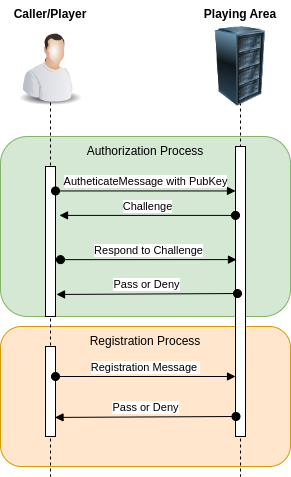
\includegraphics{AuthenticateUML.png}
\end{center}


\end{document}
